Un condensateur $C_1 = \qty{\v{C1}}{\micro\farad}$ est branché en série avec un groupe formé de $C_2 = \qty{\v{C2}}{\micro\farad}$ et $C_3 = \qty{\v{C3}}{\micro\farad}$ en parallèle. L'ensemble est relié à une pile de \qty{\v{V}}{V}.

\begin{center}
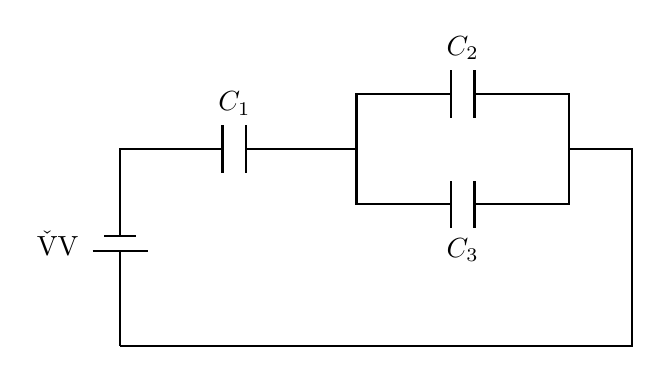
\begin{tikzpicture}[thick]
    % pile
    \draw (0,0) -- (0,1.2);
    \draw (-0.35,1.2) -- (0.35,1.2);
    \draw (-0.2,1.4) -- (0.2,1.4);
    \draw (0,1.4) -- (0,2.5) -- (1.3,2.5);
    \node[left] at (-0.4,1.3) {\qty{\v{V}}{V}};
    % C1
    \draw (1.3,2.2) -- (1.3,2.8); \draw (1.6,2.2) -- (1.6,2.8);
    \node[above] at (1.45,2.8) {$C_1$};
    \draw (1.6,2.5) -- (3,2.5);
    % parallel C2 C3
    \draw (3,2.5) -- (3,3.2) -- (4.2,3.2); \draw (3,2.5) -- (3,1.8) -- (4.2,1.8);
    \draw (4.2,2.9) -- (4.2,3.5); \draw (4.5,2.9) -- (4.5,3.5); \node[above] at (4.35,3.5) {$C_2$};
    \draw (4.2,1.5) -- (4.2,2.1); \draw (4.5,1.5) -- (4.5,2.1); \node[below] at (4.35,1.5) {$C_3$};
    \draw (4.5,3.2) -- (5.7,3.2) -- (5.7,1.8) -- (4.5,1.8);
    \draw (5.7,2.5) -- (6.5,2.5) -- (6.5,0) -- (0,0);
\end{tikzpicture}
\end{center}

\begin{enumerate}[label=\alph*)]
    \item Déterminez la capacité équivalente du montage.
    \item Déterminez la charge sur $C_1$ et la différence de potentiel à ses bornes.
    \item Déterminez la différence de potentiel aux bornes de $C_2$ et la charge sur $C_2$.
\end{enumerate}
